\section{Dataset}

We construct a large-scale optical prescription dataset for generative modeling by combining patent-derived lens designs with synthetic designs generated through controlled perturbation and post-processing of those patents. Each design is retained in two linked forms: an individual CodeV sequence file for optical simulation and a common tabular prescription row for data analysis and downstream model training. The tabular representation stores the design parameters, design conditions, material assignments, optical-performance annotations, and provenance fields needed to connect each row back to its patent source design. The patent-derived designs provide realistic reference families across surface counts, optical configurations, apertures, field angles, and material choices, while the synthetic expansion increases coverage around those families in the same tabular prescription format. The remainder of this section further expands on the details of the dataset in the following order: Section~\ref{sec:dataset_patent_reference} introduces the patent-derived reference corpus and its optical prescription representation. Section~\ref{sec:dataset_patent_shortlisting} describes the standardization and shortlisting procedure, and Section~\ref{sec:dataset_synthetic_expansion} presents the traceable synthetic expansion workflow and resulting dataset.

\subsection{Patent-Derived Reference Designs}
\label{sec:dataset_patent_reference}

The collected patent-derived reference corpus contains 2,572 optical system designs assembled from the CodeV patent library, the Zemax Zebase library, and a public file exchange for lens designs~\cite{codev,zemax_opticstudio,reiley_lens_design_exchange}. Source attribution is recorded through patent identifiers, publication citations, or the best available source record. These designs form the source pool from which the modeling-ready patent subset is selected and later synthetically expanded.

Because the source files use different optical-design formats and glass definitions, the collected prescriptions were converted to CodeV \texttt{.seq} files, including conversion of Zemax formats. Generic glass codes and obsolete or discontinued glasses were replaced with available catalog materials using the CodeV GLASSFIT procedure. LLIMAS supplied a refocusing optimization to CodeV, which adjusted the image-plane position to minimize residual defocus introduced by the material substitutions~\cite{Doyle2017LLIMAS,codev}. The design wavelengths were then normalized to the Fraunhofer F, d, and C lines (486.1, 587.56, and 656.3~nm, respectively), followed by a second CodeV refocusing operation. Each curated prescription retains its source attribution and corresponding sequence-file artifact.

{\color{red}Detailed field-condition conventions across the full 2,572-design patent-derived reference corpus will be added after the source audit is completed.}

Each optical system is represented as a sequence of surfaces with associated geometric and material parameters. Figure \ref{fig:lens_param} illustrates the lens assembly and the parameters used to define the design space. For each active surface $j$, the table records:
\begin{enumerate}
    \item \textbf{Radius of curvature $R_j$}: signed radius of curvature of surface $j$;
    \item \textbf{Thickness $t_j$}: axial distance between surfaces $j$ and $j+1$;
    \item \textbf{Material $j$}: optical material immediately following surface $j$;
    \item \textbf{Semi-diameter $h_j$}: radial aperture height of surface $j$;
    \item \textbf{Aperture stop index}: index of the surface designated as the aperture stop.
\end{enumerate}

\begin{figure}[ht]
    \centering
    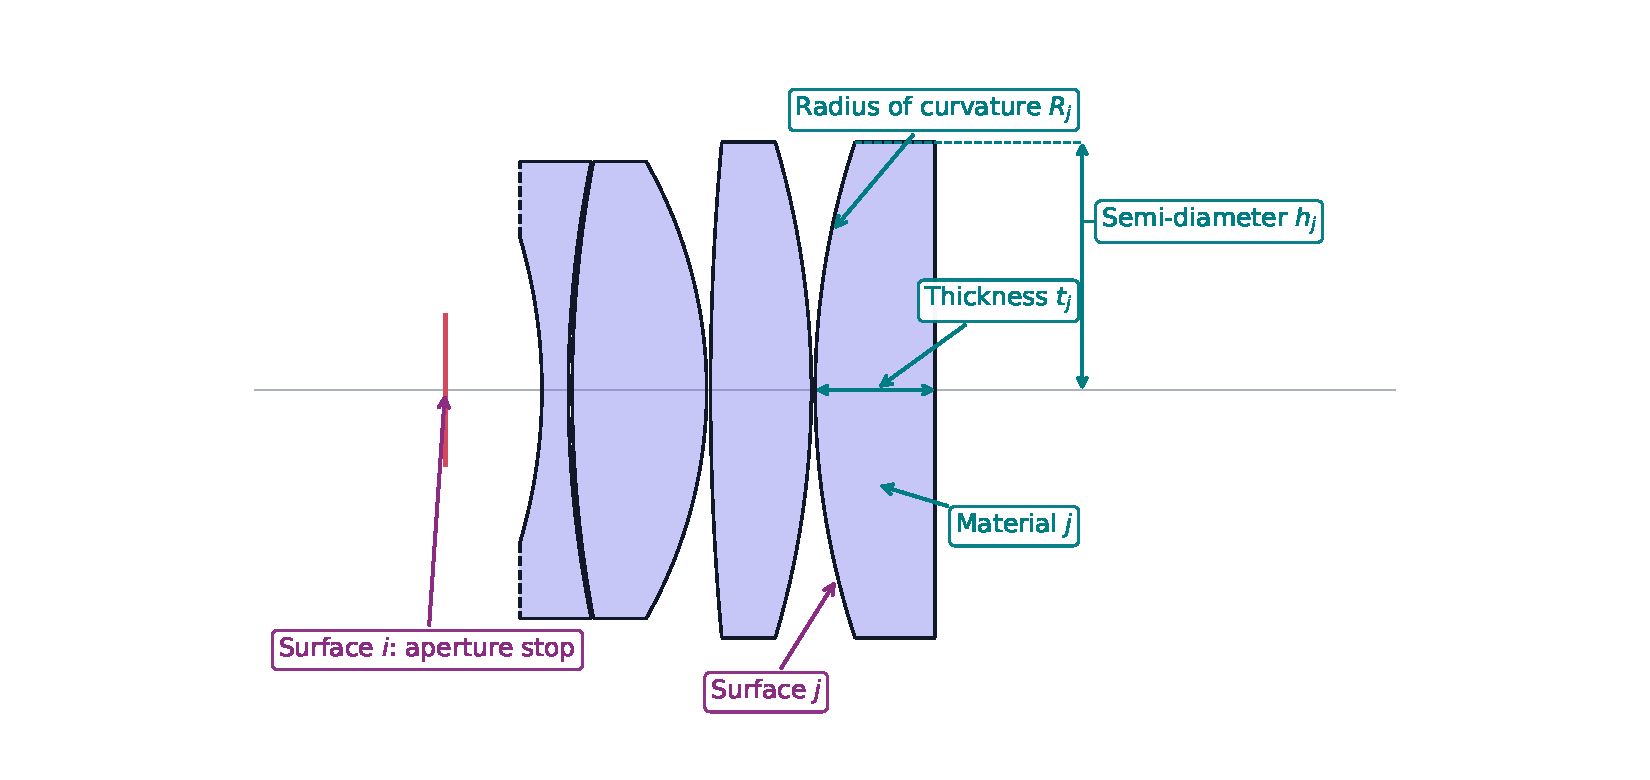
\includegraphics[width=0.85\linewidth]{figures/lens_params_def_programmatic/figure_2_patent_lens_parameters.pdf}
    \caption{\small\textbf{Lens system diagram with highlighted parameters.} A representative held-out patent-derived assembly is rendered from its prescription, with symbolic annotations for the surface radius of curvature, thickness, material, semi-diameter, surface index, and aperture-stop index used in the dataset representation.}
    \label{fig:lens_param}
\end{figure}

Along with design parameters, each optical system is associated with operating conditions that define its intended use:
\begin{enumerate}
    \item \textbf{Maximum field angle}: largest field angle to be accommodated by the system;
    \item \textbf{Effective focal length (EFL)}: target effective focal length;
    \item \textbf{Entrance pupil diameter (EPD)}: intended entrance pupil diameter;
    \item \textbf{Total length}: axial distance from the first surface to the image plane.
\end{enumerate}

The dataset also retains optical-performance annotations. The annotations used in this study include:
\begin{enumerate}
    \item \textbf{Spot-size metrics}: field-dependent spot-size measures such as SPO67 and SPO100;
    \item \textbf{Encircled-energy metrics}: field-dependent energy-concentration measures such as EE50 and EE90;
    \item \textbf{Axial nominal performance}: on-axis root-mean-square (RMS) wavefront error.
\end{enumerate}
Additional performance and sensitivity annotations are retained in the canonical dataset.\\
{\color{red}A complete inventory of the retained performance and sensitivity annotations will be added after the metric audit is completed.}
Unless otherwise specified, distances are reported in millimeters, angles in degrees, and wavelengths in nanometers.

\subsection{Patent Dataset Shortlisting}
\label{sec:dataset_patent_shortlisting}

To formulate a standardized starting point for generative modeling and synthetic dataset generation, we select and process designs from the collected reference corpus according to the following standardization and filtering criteria:
\begin{enumerate}
    \item Designs are specified for object distance of infinity.
    \item Materials are selected from existing optical material catalogues.
    \item Object and image spaces are air.
    \item Object and image surfaces are represented as flat/planar surfaces without curvature.
    \item Aspheric surfaces and gratings are not considered.
    \item The number of surfaces ranges from 3 to 17.
    \item A maximum field angle is used as a design specification.
    \item Design performance is evaluated at $\{0, 0.3, 0.5, 0.7, 1.0\}$ times the maximum field angle.
    \item Field angles are represented in the meridional/y-field direction, with x-field angle entries set to zero.
    \item Performance is evaluated in the visible spectrum using fixed wavelengths (F, d, C lines).
    \item The material between the last surface and image plane is air, and the penultimate material is glass.
\end{enumerate}

Applying these criteria gives a canonical subset of 1,253 confirmed patent designs selected from the broader 2,572-design patent-derived reference corpus. The retained rows keep the same tabular optical-prescription schema as the curated source corpus: non-applicable or structurally irrelevant cells are left empty, while fields affected by the standardization criteria are updated to the canonical form used for synthetic generation and modeling.\\
{\color{red}Detailed shortlisting counts from the collected patent corpus to the canonical patent subset need to be added after the source audit is finalized.}

\subsection{Synthetic Expansion}
\label{sec:dataset_synthetic_expansion}

The synthetic dataset is generated from the canonical patent subset using perturbations that preserve the tabular prescription format described above. This expansion is intended to increase the number and coverage of available optical prescriptions while keeping each synthetic row traceable to a realistic patent-derived design family. At a high level, the synthetic construction process is:
\begin{enumerate}
    \item sample a parent design from the canonical patent subset;
    \item perturb curvature, thickness, material, or combinations of these quantities;
    \item re-evaluate semi-diameters and image-plane placement using the optical evaluation pipeline;
    \item discard rows that fail the generation or simulation checks;
    \item retain successful rows with full lineage back to the parent design and perturbation source.
\end{enumerate}
Figure~\ref{fig:synth_data_pipe} summarizes this synthetic dataset construction workflow.

\begin{figure}[ht]
    \centering
    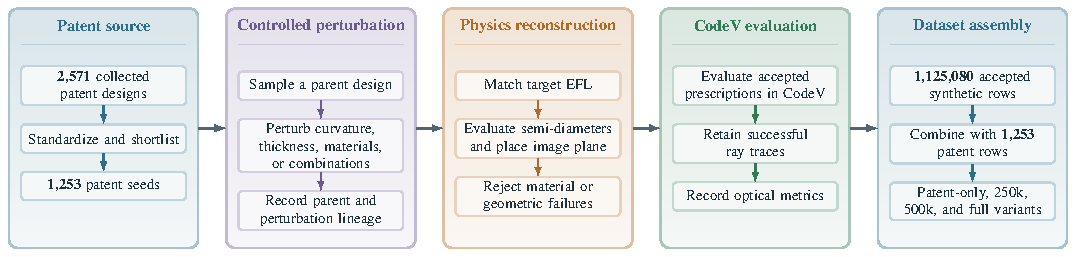
\includegraphics[width=\linewidth]{figures/synthetic_dataset_pipeline_tikz.pdf}
    \caption{\small\textbf{Synthetic dataset construction pipeline.} Patent-derived designs are standardized and shortlisted, perturbed with parent and perturbation lineage retained, reconstructed and filtered using optical checks, evaluated in CodeV, and assembled into the Patent-only, 250k, 500k, and full study datasets. Colors denote data artifacts (teal), controlled perturbation (purple), physics reconstruction (orange), and CodeV evaluation (green); arrows indicate forward data flow.}
    \label{fig:synth_data_pipe}
\end{figure}

The resulting canonical dataset contains 1,126,333 rows: 1,253 patent-derived rows and 1,125,080 synthetic rows. The synthetic rows are retained in the same tabular prescription format as the patent-derived rows and are generated through curvature, thickness, material, and combined perturbation families. Provenance fields are retained so that synthetic rows can be traced back to their parent patent designs and perturbation sources.

Figure \ref{fig:patent_synth_comp} summarizes patent-derived and synthetic dataset characteristics. Additional surface-count, condition-range, remaining-field optical-performance, and perturbation-lineage figures are provided in Appendix~\ref{app:dataset_details}, including Figure~\ref{fig:appendix_remaining_field_performance}.

\begin{figure}[t]
    \centering
    \begin{subfigure}[t]{0.48\linewidth}
        \centering
        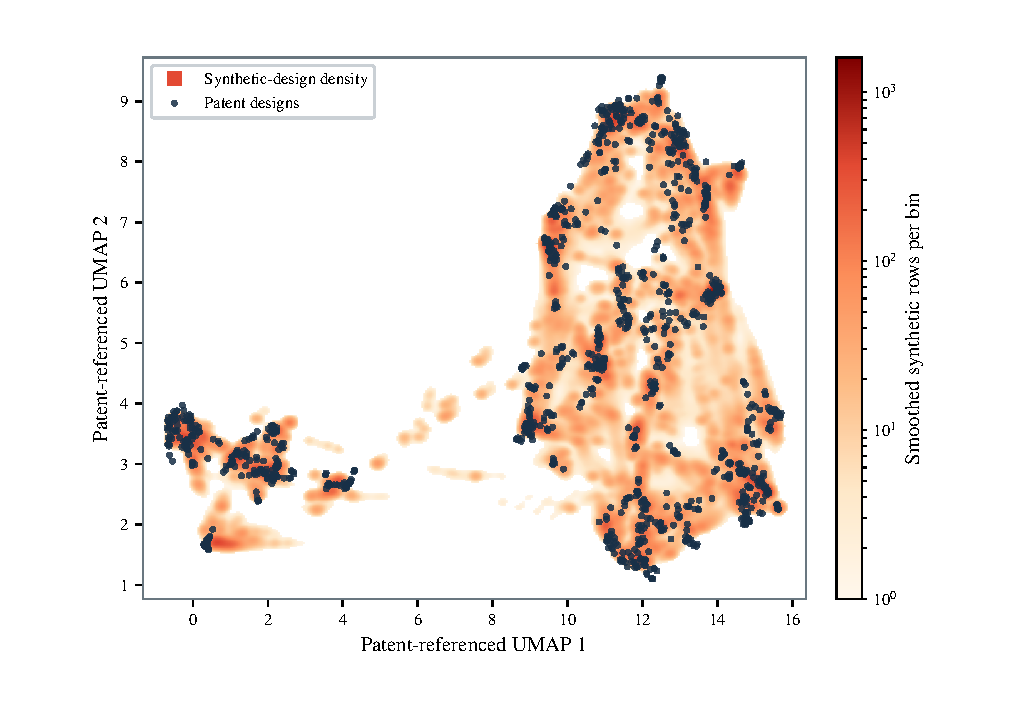
\includegraphics[width=\linewidth]{figures/mixed_landmark_umap_projection.pdf}
        \caption{Patent-referenced tuned-representation projection}
        \label{fig:patent_synth_comp_div}
    \end{subfigure}
    \hfill
    \begin{subfigure}[t]{0.48\linewidth}
        \centering
        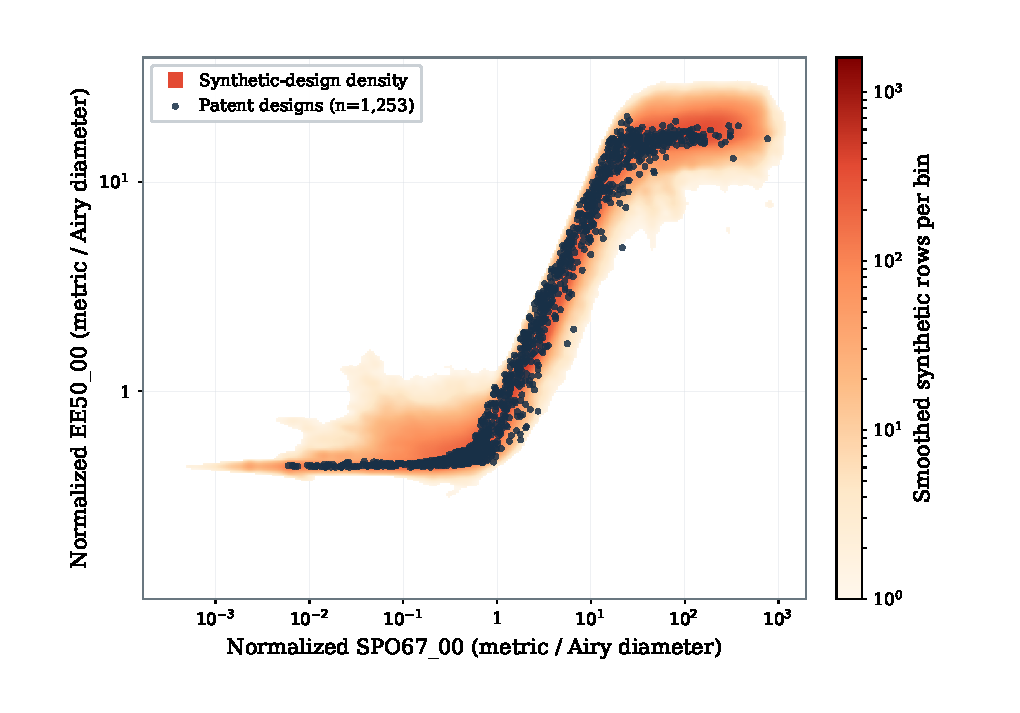
\includegraphics[width=\linewidth]{figures/normalized_ee50_vs_spo67.pdf}
        \caption{Normalized EE50 versus SPO67 comparison}
        \label{fig:patent_synth_comp_perf}
    \end{subfigure}
    \caption{\small\textbf{Patent-derived and synthetic dataset comparison.} Left: topology-aware projection used to compare coverage of patent-derived and synthetic designs. Right: normalized encircled-energy and spot-size comparison for optical-performance characterization.}
    \label{fig:patent_synth_comp}
\end{figure}
